\documentclass[12pt,a4paper]{article}
\usepackage[T1]{fontenc}
\usepackage[a4paper]{geometry}
\usepackage[portuges,brazilian]{babel}
\usepackage[utf8]{inputenc}
\usepackage{setspace}
\usepackage{libertine}
\usepackage{graphicx}	
\usepackage{ragged2e} 
\usepackage{authblk}
\usepackage{hyperref}	
\usepackage{amsmath}	
\usepackage{tikz}
%
\newcommand*{\email}[1]{%
    \normalsize\href{mailto:#1}{#1}\par
    }


\begin{document} 
\begin{figure}
    \flushright
    
\includegraphics[scale=0.5]{Logo_senai.png}
\end{figure}

\title{Estudo estatístico \\ Análise de Regressão} 
\author{Anderson Queiroz  \\ Rodrigo Formiga}
\affil{Senai Cimatec. CCRoSA - Centro de Competência em Robótica e Sitemas Autônomos \\ \email{anderson.vale@fbter.org.br \\ rodrigo.farias@fbter.org.br}}

 

    \maketitle
    \pagenumbering{arabic}
    \singlespacing

    \section{Introdução}

O experimento apresentado neste relatório consistiu em avaliar a influência de dois parâmetros básicos no tempo de queda de alguns modelos de ``helicóptero'' feito em dobraduras de papel.

\subsection{\textit{Six Sigma}}

A filosofia \textit{Six Sigma} (ou Seis Sigma) é uma estratégia em que você define rotinas e desenvolve trabalhos de melhoria de processos em sua organização \cite{sixsigma}. Este método foi originado pelo programa de melhoria da qualidade da Motorola em 1987 com o objetivo de se aproximar do zero defeito. Com o sucesso alcançado pela metodologia na empresa, o processo foi difundido \cite{correa}. \textit{Six Sigma} trabalha com três grandes objetivos: redução de custos, otimização de processos e satisfação do cliente \cite{sixsigma}.

Tendo em vista essa informação, existe uma escala que determina a qualidade do processo:

\begin{figure}[h]
  \centering
  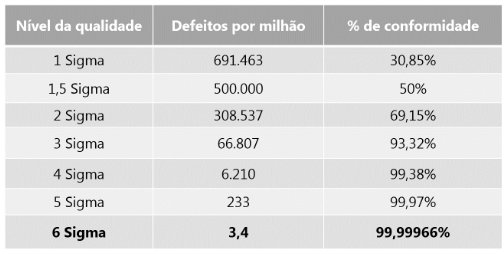
\includegraphics[scale=0.7]{images/tabless.png}
  \caption{Tabela \emph{Six Sigma} \cite{sixsigma}}
  \label{fig:sixsigma}
\end{figure}

A partir da tabela, podemos perceber o espectro de algumas empresas, que trabalham em produção de milhões de unidades, então obter somente 99\% de confiabilidade não é o bastante. O processo é definido como 6 Sigma ao atingir uma proporção de 3 ou 4 erros a cada 1 milhão de unidades produzidas. Algumas empresas aceitam trabalhar como 4 Sigma em alguns dos seus processos.

\subsection{Otimização de Processos}

A otimização de respostas em um processo é fundamental para o \textit{Six Sigma} na fase de melhoria. Uma das ferramentas mais importantes que representa o conceito principal dessa filosofia é a Planejamento de Experimentos (\textbf{DoE}). \textbf{DoE} busca combinar fatores de um processo com o objetivo de otimizar a resposta desejada extraindo o máximo possível de informações com um número mínimo de experimentos. \cite{abepro}

O planejamento e a condução desses testes também fazem parte do \textbf{DoE}, visto que a falta de planejamento ou a má condução pode culminar em resultados incoerentes, obrigando a repetição de todo o processo de análise, ou mesmo falsos-positivos. Os testes devem ser projetados de modo que a aleatoriedade esteja sempre presente, em detrimento a qualquer eventual manipulação dos dados, pois ela é uma peça fundamental na normalidade dos experimentos. % Jean
	\section{Revisão literária}

Serão apresentados na presente seção alguns pontos que, segundo a literatura, nortearão o estudo estatístico do trabalho em questão, abordando alguns pontos importantes para realização do planejamento e análise dos experimentos. Logo em seguida, serão aplicados os conceitos aqui apresentados.


\subsection{Planejamento e análise de experimentos}

Técnicas de planejamento e análises de experimentos são utilizáveis em empresa, processo de fabricação, desenvolvimento de um novo produto e até em fabricação de commodities. Geralmente a maioria destes processos possuem diversas variáveis controláveis, como temperatura, velocidade, dimensões entre outras. A variação destas variáveis, de modo isolado ou combinado, pode trazer melhorias ou prejuízos a qualidade do produto ou serviço. Com isso, faz-se necessário um estudo analítico de como cada variável pode influenciar o processo \cite{1}. 

O planejamento e análise de experimentos (\textit{Design of Experiments, \textbf{DOE}}) é uma técnica de planejamento de experimentos, ou seja, como os experimentos devem proceder para garantir conclusões assertivas. A validade das conclusões obtidas após análise dos experimentos, são diretamente ligadas ao modo como os experimentos foram realizados, logo, o planejamento do experimento torna-se o ponto mais importante na hora de se analisar algum processo produtivo, bens ou serviços prestados. O planejamento corretamente executado também pode evitar desperdícios, além de isolar e determinar relações das variáveis \cite{1}.

A seguir serão apresentados alguns pontos importantes para análise estatística realizada neste presente trabalho, como: Princípios do planejamento, que irão nortear como deve ser condizido o planejamento de experimentos, bem como etapas para realização dos experimentos e análise dos mesmos \cite{2}.


\subsubsection{Princípios do planejamento de experimentos}

O planejamento de experimentos possui três principais princípios básicos, que são: Replicação, aleatóriedade e blocagem \cite{2}. 

\subsubsection*{Replicação}

A replicação consiste na obtenção de mais de uma unidade experimental, ou seja, replicar o teste para cada ponto experimental e assim permite que obtenha-se uma estimativa mais precisa, diminuindo a influência de variações indesejadas ou inevitáveis \cite{2}.

\subsubsection*{Aleatóriedade}

Os métodos estatísticos requerem que as observações sejam variáveis aleatórias, de modo a garantir a distribuição igual dos fatores não esperados. Com isso garantem-se estimativas não tendênciosas dos efeitos e erros experimentais, bem como evitar influência sistemática de fatores não controláveis \cite{2}. 
\subsubsection*{Blocagem}

A blocagem é uma técnica extremamente importante, utilizada com o objetivo de aumentar a precisão de um experimento. Este princípio pode ser aplicado em alguns casos onde deseja-se isolar algum fator conhecido, analisando de forma individual sua influência sobre o processo. A mudança de pessoas no processo experimental ou a mudança de lote de um produto pode ser visto a princípio como um fator não desejado de ser analisado, logo, o princípio de blocagem permite que o mesmo seja isolado, porém, não ignorado\cite{2}. 

\subsubsection{Etapas para o desenvolvimento de experimentos}

Coleman e Montgomery (1993) propõem as seguintes etapas para o desenvolvimento de um planejamento de experimentos \cite{3}:

\begin{enumerate}
    \item \textbf{Caracterização do problema:}
    A definição do problema que está sendo analisado é uma etapa essencial para se entender o estudo analítico. Para isso se faz necessário conhecimento sobre todo o processo para assim definir de forma clara o objetivo e relatar de forma específica o problema analisado.

    \item \textbf{Escolha dos fatores de influência e níveis:}
    Para conduzir o experimento deve-se escolher os fatores variáveis, os intervalos sobre os quais esses fatores variarão e os níveis específicos. Para tanto é necessário conhecimento do processo, experiências práticas e teóricas para determinar tais fatores mais relevantes para análise experimental.
    \item \textbf{Seleção das variáveis de resposta:}
    É também necessário ao planejar um experimento que se tenha clareza de qual variável-resposta será obtida como parâmetro para qualificar os experimentos. Variável de resposta que não atenda a necessidade do experimento pode levar a conclusões equivocadas. 
    \item \textbf{Determinação de um modelo de planejamento de experimento:}
    A escolha do planejamento envolve consideração sobre o tamanho da amostra (número de replicações) e determinar se há formação de blocos ou outras restrições de aleatorização.
    \item \textbf{Condução do experimento:}
    A condução do experimento deve seguir todo o planejamento, evitando variações de ambiente, métodologia do experimento ou inserção de novas variações não previamente estabelecidas. O responsável pelo experimento e os equipamentos utilizados devem ser mantidos do início ao fim, exceto em casos onde estas variações sejam desejáveis.

    \item \textbf{Análise dos dados:}
    
    Após todas as demais etapas anteriores, os resultados podem ser obtidos com uso de ferramentas e pacotes estatísticos para auxiliar na visualização de gráficos e dados. A verificação da validade do modelo é também um ponto importante para análisar. 

    \item \textbf{Conclusões e recomendações:}
    
    Após a obtenção dos resultados, o experimento deve apresentar conclusões práticas para proporcionar recomendações de ações em cima do processo analisado. As recomendações são frutos das etapas decorridas no planejamento do experimento, ou seja, planejamentos com falhas iram gerar ações equivocadas no processo. 
     
\end{enumerate}

\subsection{Análise de regressão}

Um método muito utilizado nos estudos estatísticos é a análise de regressão, este método permite examinar a relação entre duas ou mais variáveis que se deseja estudar. O método permite por meio de modelos matemáticos avaliar quais as relações entre as variáveis, quais delas são importantes para o processo e quais apresentam pouca relevância \cite{4}. 

As variáveis utilizadas podem ser divididas em duas: Variável Dependente, que é a variável que está sendo estudada, como uma sáida do processo (a influência das demais variáveis será analisada através das variáveis dependentes); e Variável Independente, que são as entradas do estudo, são variáveis que supostamente causam impactos ou certa influência na variável dependente \cite{4}.

A análise de regressão tem por finalidade chegar a algumas conclusões e direcionamentos sobre o processo estudado, as finalidades deste estudo são \cite{4}:

\begin{itemize}
    \item Predição dos dados;
    \item Seleção de variáveis influenciáveis no processo;
    \item Estimação de parâmetros;
    \item Realizar inferências sobre os parâmetros, como: testes de hipóteses e intervalos de confiança.
\end{itemize}

% http://cursos.leg.ufpr.br/ce072/slides-pdf/01-planej-revisao.pdf
% http://www.portalaction.com.br/planejamento-de-experimento/introducao#:~:text=Tr%C3%AAs%20princ%C3%ADpios%20b%C3%A1sicos%20de%20um,blocagem.
% http://www.portaldeconhecimentos.org.br/index.php/por/Conteudo/Planejamento-de-Experimentos-DOE
% http://www.dpi.ufv.br/~peternelli/inf162.www.16032004/materiais/CAPITULO9.pdf % Rodrigo
	\section{Resultados}

A partir dos testes realizados sob orientação do planejamento, anteriormente mencionado na seção X, foram coletados os resultados do tempo de vôo do helicóptero. As amostras dos testes coletados, como pode ser visto na tabela \ref{tab:amostras}, possui os seguintes parâmetros: \textbf{clipe} que pode ser com ou sem; \textbf{AT} que representa o adesivo no topo do helicóptero, sendo com ou sem; \textbf{ADLat} é o adesivo lateral, podendo ser colocado o adesivo do lado direito ou do lado esquerdo; \textbf{AL} é a altura de partida do helicóptero, em que foi definido como 1,30 m e 2,10 m e o tempo de queda em segundos. Dessa forma, com base nestes valores de tempo, a partir das disposições dos demais parâmetros, foi feito o teste de regressão para analisar a influência da relação entre os parâmetros com o tempo.

\begin{table}[ht]
    \centering
    \caption{Resultados das amostras coletadas.}
    \begin{tabular}{rllllr}
      \hline
     & clip & AT & ADLat & AL & tempo \\ 
      \hline
    1 & S & S & E & 1.30 & 0.92 \\ 
      2 & C & S & E & 1.30 & 0.88 \\ 
      3 & S & C & E & 1.30 & 1.04 \\ 
      4 & C & C & E & 1.30 & 1.10 \\ 
      5 & S & S & D & 1.30 & 1.10 \\ 
      6 & C & S & D & 1.30 & 0.99 \\ 
      7 & S & C & D & 1.30 & 1.07 \\ 
      8 & C & C & D & 1.30 & 0.92 \\ 
      9 & S & S & E & 2.10 & 1.76 \\ 
      10 & C & S & E & 2.10 & 1.23 \\ 
      11 & S & C & E & 2.10 & 1.88 \\ 
      12 & C & C & E & 2.10 & 1.52 \\ 
      13 & S & S & D & 2.10 & 1.70 \\ 
      14 & C & S & D & 2.10 & 1.72 \\ 
      15 & S & C & D & 2.10 & 1.46 \\ 
      16 & C & C & D & 2.10 & 1.42 \\ 
       \hline
    \end{tabular}
    \label{tab:amostras}
\end{table}

A análise de regressão deste sistema foi divida em 2 modelos: primeira e segunda ordem. Como o sistema possui 4 variáveis independentes, o modelo máximo atingido pode ser representado pela relação entre os 4 parâmetros. Porém, a partir do terceiro modelo não há mais significância entre os resultados obtidos, que será mostrado em diante, descartando assim a análise com um número maior de relações. 

\subsection{Análise de Primeira Ordem - Modelo 1}

A partir da análise linear aplicada aos resultados das amostras, aplicando-se a primeira ordem, o resultado é mostrado na tabela \ref{tab:model1}. O primeiro modelo dessa análise pode ser visualizado na Equação \ref{eq:model1}. Esta equação mostra um modelo que consegue explicar o valor do tempo a partir da relação entre os parâmetros. Os valores dentro dos parâmetros são as variáveis que mais apresentaram valores significantes ao sistema, dentre as opções estabelecidas. 

\begin{table}[ht]
    \centering
    \caption{Resultado da análise linear de primeira ordem do modelo 1.}
    \begin{tabular}{rrrrr}
      \hline
     & Estimate & Std. Error & t value & Pr($>$$|$t$|$) \\ 
      \hline
    (Intercept) & 1.0622 & 0.0910 & 11.67 & 1.54e-07 \\ 
      clipC & -0.1419 & 0.0814 & -1.74 & 0.1092 \\ 
      ATC & 0.0119 & 0.0814 & 0.15 & 0.8866 \\ 
      ADLatD & 0.0081 & 0.0814 & 0.10 & 0.9223 \\ 
      AL2.10 & 0.5844 & 0.0814 & 7.18 & 1.80e-05 \\ 
       \hline
    \end{tabular}
    \label{tab:model1}
\end{table}

\begin{align}
    \begin{split}
    tempo &= 1.062187 - 0.141875\text{.clip(C)} + 0.011875\text{.AT(C)} \\
    & + 0.008125\text{.ADLat(D)} + 0.584375\text{.AL2,10}
    \end{split}
    \label{eq:model1}
\end{align}

Com base na tabela\ref{tab:model1}, pode ser visto que estatisticamente os estimadores dos parâmetros clipe, AT e ADLat são iguais a zero, pois, ao se assumir o nível de significância a 5\% de probabilidade, o $\rho$ valor desses coeficientes é superior a 0,05, aceitando a hipótese nula, ou seja, as estimativas desses parâmetros são números muitos próximos de zero no qual pelo teste t afirma-se que esses valores aceitam a hipótese $H_0$. Portanto, se os parâmetros clipe, AT e ADLat são estatisticamente iguais a zero, eles não precisam estar no modelo pois não vai ter nenhuma contribuição significante no valor de tempo de queda do helicóptero. Então, o novo modelo pode ser representado na equação \ref{eq2:model1}, refazendo-se a análise linear do tempo de queda com relação apenas ao parâmetro AL. O resultado dos coeficientes pode ser visto na tabela\ref{tab:model1}. 

\begin{table}[ht]
    \centering
    \caption{Análise linear da relação do tempo com AL.}
    \begin{tabular}{rrrrr}
      \hline
     & Estimate & Std. Error & t value & Pr($>$$|$t$|$) \\ 
      \hline
    (Intercept) & 1.0012 & 0.0577 & 17.35 & 7.29e-11 \\ 
      AL2.10 & 0.5844 & 0.0816 & 7.16 & 4.84e-06 \\ 
       \hline
    \end{tabular}
    \label{tab2:model1}
\end{table}

\begin{align}
    tempo = 1.00125 + 0.58438\text{.AL2,10}
    \label{eq2:model1}
\end{align}

O modelo apresentado na equação \ref{eq:model1}, que representa uma regressão múltipla, foi reduzido para uma regressão simples, representado pela equação \ref{eq2:model1}. Desse modo, para explicar a equação reduzida pode-se dizer que para cada acréscimo a partir da altura de 2,10 m, o tempo de queda aumenta em 0,58 s. Com base no valor do $R^2$, que foi de 78,56\%, pode se afirmar a porcentagem do dados que são explicados pelo modelo da equação \ref{eq2:model1}. O valor do $R^2$ ajustado será desconsiderado pois esse último modelo foi o único em que todos os estimadores dos parâmetros foram significativos, no caso dessa análise linear do modelo 1. 

Analisando os resíduos do modelo 1 simplificado, foi aplicado o teste de normalidade de \textit{Shapiro-Wilk}. Nesse teste pode-se afirmar que, a partir da verificação dos resíduos desse modelo mostrou-se que no teste da normalidade apresentou um valor de 0,97528 com o $\rho$ valor respectivo de 0,9152, e adotando o nível de significância de 5\%, não houve violação da normalidade dos resíduos. Então, pode-se concluir que esses erros (resíduos) tem uma distribuição normal, como pode ser visto nos gráficos das figuras \ref{fig:qq} e \ref{fig:hist}. Dessa forma, assume-se a independência dos resíduos pelo fato que a estrutura de coleta declara essa independência. Portanto, não é preciso atribuir testes de independência.

\begin{figure}
    \centering
    \caption{Distribuição normal dos resíduos.}
    % Created by tikzDevice version 0.12.3 on 2020-09-22 19:17:36
% !TEX encoding = UTF-8 Unicode
\begin{tikzpicture}[x=1pt,y=1pt]
\definecolor{fillColor}{RGB}{255,255,255}
\path[use as bounding box,fill=fillColor,fill opacity=0.00] (0,0) rectangle (308.44,270.16);
\begin{scope}
\path[clip] ( 49.20, 61.20) rectangle (283.24,220.96);
\definecolor{drawColor}{RGB}{0,0,0}

\path[draw=drawColor,line width= 0.4pt,line join=round,line cap=round] (132.53,128.22) circle (  2.25);

\path[draw=drawColor,line width= 0.4pt,line join=round,line cap=round] (107.47,118.98) circle (  2.25);

\path[draw=drawColor,line width= 0.4pt,line join=round,line cap=round] (170.78,155.96) circle (  2.25);

\path[draw=drawColor,line width= 0.4pt,line join=round,line cap=round] (189.62,170.98) circle (  2.25);

\path[draw=drawColor,line width= 0.4pt,line join=round,line cap=round] (199.91,170.98) circle (  2.25);

\path[draw=drawColor,line width= 0.4pt,line join=round,line cap=round] (161.66,146.71) circle (  2.25);

\path[draw=drawColor,line width= 0.4pt,line join=round,line cap=round] (180.02,164.05) circle (  2.25);

\path[draw=drawColor,line width= 0.4pt,line join=round,line cap=round] (142.82,129.38) circle (  2.25);

\path[draw=drawColor,line width= 0.4pt,line join=round,line cap=round] (242.89,188.46) circle (  2.25);

\path[draw=drawColor,line width= 0.4pt,line join=round,line cap=round] ( 57.87, 67.12) circle (  2.25);

\path[draw=drawColor,line width= 0.4pt,line join=round,line cap=round] (274.57,215.04) circle (  2.25);

\path[draw=drawColor,line width= 0.4pt,line join=round,line cap=round] (152.42,132.99) circle (  2.25);

\path[draw=drawColor,line width= 0.4pt,line join=round,line cap=round] (211.38,174.59) circle (  2.25);

\path[draw=drawColor,line width= 0.4pt,line join=round,line cap=round] (224.97,179.21) circle (  2.25);

\path[draw=drawColor,line width= 0.4pt,line join=round,line cap=round] (121.06,119.12) circle (  2.25);

\path[draw=drawColor,line width= 0.4pt,line join=round,line cap=round] ( 89.55,108.72) circle (  2.25);
\end{scope}
\begin{scope}
\path[clip] (  0.00,  0.00) rectangle (308.44,270.16);
\definecolor{drawColor}{RGB}{0,0,0}

\path[draw=drawColor,line width= 0.4pt,line join=round,line cap=round] ( 49.88, 61.20) -- (282.56, 61.20);

\path[draw=drawColor,line width= 0.4pt,line join=round,line cap=round] ( 49.88, 61.20) -- ( 49.88, 55.20);

\path[draw=drawColor,line width= 0.4pt,line join=round,line cap=round] (108.05, 61.20) -- (108.05, 55.20);

\path[draw=drawColor,line width= 0.4pt,line join=round,line cap=round] (166.22, 61.20) -- (166.22, 55.20);

\path[draw=drawColor,line width= 0.4pt,line join=round,line cap=round] (224.39, 61.20) -- (224.39, 55.20);

\path[draw=drawColor,line width= 0.4pt,line join=round,line cap=round] (282.56, 61.20) -- (282.56, 55.20);

\node[text=drawColor,anchor=base,inner sep=0pt, outer sep=0pt, scale=  1.00] at ( 49.88, 39.60) {-2};

\node[text=drawColor,anchor=base,inner sep=0pt, outer sep=0pt, scale=  1.00] at (108.05, 39.60) {-1};

\node[text=drawColor,anchor=base,inner sep=0pt, outer sep=0pt, scale=  1.00] at (166.22, 39.60) {0};

\node[text=drawColor,anchor=base,inner sep=0pt, outer sep=0pt, scale=  1.00] at (224.39, 39.60) {1};

\node[text=drawColor,anchor=base,inner sep=0pt, outer sep=0pt, scale=  1.00] at (282.56, 39.60) {2};

\path[draw=drawColor,line width= 0.4pt,line join=round,line cap=round] ( 49.20, 77.59) -- ( 49.20,218.72);

\path[draw=drawColor,line width= 0.4pt,line join=round,line cap=round] ( 49.20, 77.59) -- ( 43.20, 77.59);

\path[draw=drawColor,line width= 0.4pt,line join=round,line cap=round] ( 49.20,112.88) -- ( 43.20,112.88);

\path[draw=drawColor,line width= 0.4pt,line join=round,line cap=round] ( 49.20,148.16) -- ( 43.20,148.16);

\path[draw=drawColor,line width= 0.4pt,line join=round,line cap=round] ( 49.20,183.44) -- ( 43.20,183.44);

\path[draw=drawColor,line width= 0.4pt,line join=round,line cap=round] ( 49.20,218.72) -- ( 43.20,218.72);

\node[text=drawColor,rotate= 90.00,anchor=base,inner sep=0pt, outer sep=0pt, scale=  1.00] at ( 34.80, 77.59) {-2};

\node[text=drawColor,rotate= 90.00,anchor=base,inner sep=0pt, outer sep=0pt, scale=  1.00] at ( 34.80,112.88) {-1};

\node[text=drawColor,rotate= 90.00,anchor=base,inner sep=0pt, outer sep=0pt, scale=  1.00] at ( 34.80,148.16) {0};

\node[text=drawColor,rotate= 90.00,anchor=base,inner sep=0pt, outer sep=0pt, scale=  1.00] at ( 34.80,183.44) {1};

\node[text=drawColor,rotate= 90.00,anchor=base,inner sep=0pt, outer sep=0pt, scale=  1.00] at ( 34.80,218.72) {2};

\path[draw=drawColor,line width= 0.4pt,line join=round,line cap=round] ( 49.20, 61.20) --
	(283.24, 61.20) --
	(283.24,220.96) --
	( 49.20,220.96) --
	( 49.20, 61.20);
\end{scope}
\begin{scope}
\path[clip] (  0.00,  0.00) rectangle (308.44,270.16);
\definecolor{drawColor}{RGB}{0,0,0}

\node[text=drawColor,anchor=base,inner sep=0pt, outer sep=0pt, scale=  1.20] at (166.22,241.42) {\bfseries Distribuicao Normal};

\node[text=drawColor,anchor=base,inner sep=0pt, outer sep=0pt, scale=  1.00] at (166.22, 15.60) {Theoretical Quantiles};

\node[text=drawColor,rotate= 90.00,anchor=base,inner sep=0pt, outer sep=0pt, scale=  1.00] at ( 10.80,141.08) {Sample Quantiles};
\end{scope}
\begin{scope}
\path[clip] ( 49.20, 61.20) rectangle (283.24,220.96);
\definecolor{drawColor}{RGB}{0,0,0}

\path[draw=drawColor,line width= 0.4pt,line join=round,line cap=round] ( 49.20, 80.41) -- (283.24,217.42);
\end{scope}
\begin{scope}
\path[clip] (  0.00,  0.00) rectangle (308.44,270.16);
\definecolor{drawColor}{RGB}{0,0,0}

\path[draw=drawColor,line width= 0.4pt,line join=round,line cap=round] ( 49.88, 61.20) -- (282.56, 61.20);

\path[draw=drawColor,line width= 0.4pt,line join=round,line cap=round] ( 49.88, 61.20) -- ( 49.88, 55.20);

\path[draw=drawColor,line width= 0.4pt,line join=round,line cap=round] (108.05, 61.20) -- (108.05, 55.20);

\path[draw=drawColor,line width= 0.4pt,line join=round,line cap=round] (166.22, 61.20) -- (166.22, 55.20);

\path[draw=drawColor,line width= 0.4pt,line join=round,line cap=round] (224.39, 61.20) -- (224.39, 55.20);

\path[draw=drawColor,line width= 0.4pt,line join=round,line cap=round] (282.56, 61.20) -- (282.56, 55.20);

\path[draw=drawColor,line width= 0.4pt,line join=round,line cap=round] ( 49.20, 77.59) -- ( 49.20,218.72);

\path[draw=drawColor,line width= 0.4pt,line join=round,line cap=round] ( 49.20, 77.59) -- ( 43.20, 77.59);

\path[draw=drawColor,line width= 0.4pt,line join=round,line cap=round] ( 49.20,112.88) -- ( 43.20,112.88);

\path[draw=drawColor,line width= 0.4pt,line join=round,line cap=round] ( 49.20,148.16) -- ( 43.20,148.16);

\path[draw=drawColor,line width= 0.4pt,line join=round,line cap=round] ( 49.20,183.44) -- ( 43.20,183.44);

\path[draw=drawColor,line width= 0.4pt,line join=round,line cap=round] ( 49.20,218.72) -- ( 43.20,218.72);
\end{scope}
\begin{scope}
\path[clip] ( 49.20, 61.20) rectangle (283.24,220.96);
\definecolor{drawColor}{RGB}{0,0,0}

\path[draw=drawColor,line width= 0.4pt,line join=round,line cap=round] ( 49.20,148.16) -- (283.24,148.16);
\end{scope}
\begin{scope}
\path[clip] (  0.00,  0.00) rectangle (308.44,270.16);
\definecolor{drawColor}{RGB}{0,0,0}

\path[draw=drawColor,line width= 0.4pt,line join=round,line cap=round] (  0.00,  0.00) --
	(308.44,  0.00) --
	(308.44,270.16) --
	(  0.00,270.16) --
	(  0.00,  0.00);
\end{scope}
\end{tikzpicture}

    \label{fig:qq}
\end{figure}

\begin{figure}
    \centering
    \caption{Histograma dos resíduos.}
    % Created by tikzDevice version 0.12.3 on 2020-09-22 19:19:05
% !TEX encoding = UTF-8 Unicode
\begin{tikzpicture}[x=1pt,y=1pt, scale=0.9]
\definecolor{fillColor}{RGB}{255,255,255}
\path[use as bounding box,fill=fillColor,fill opacity=0.00] (0,0) rectangle (308.44,270.16);
\begin{scope}
\path[clip] (  0.00,  0.00) rectangle (308.44,270.16);
\definecolor{drawColor}{RGB}{0,0,0}

\node[text=drawColor,anchor=base,inner sep=0pt, outer sep=0pt, scale=  1.20] at (166.22,241.42) {\bfseries Histograma dos Resíduos};

\node[text=drawColor,anchor=base,inner sep=0pt, outer sep=0pt, scale=  1.00] at (166.22, 15.60) {Resíduos};

\node[text=drawColor,rotate= 90.00,anchor=base,inner sep=0pt, outer sep=0pt, scale=  1.00] at ( 10.80,141.08) {Frequência};
\end{scope}
\begin{scope}
\path[clip] (  0.00,  0.00) rectangle (308.44,270.16);
\definecolor{drawColor}{RGB}{0,0,0}

\path[draw=drawColor,line width= 0.4pt,line join=round,line cap=round] ( 57.87, 61.20) -- (274.57, 61.20);

\path[draw=drawColor,line width= 0.4pt,line join=round,line cap=round] ( 57.87, 61.20) -- ( 57.87, 55.20);

\path[draw=drawColor,line width= 0.4pt,line join=round,line cap=round] (101.21, 61.20) -- (101.21, 55.20);

\path[draw=drawColor,line width= 0.4pt,line join=round,line cap=round] (144.55, 61.20) -- (144.55, 55.20);

\path[draw=drawColor,line width= 0.4pt,line join=round,line cap=round] (187.89, 61.20) -- (187.89, 55.20);

\path[draw=drawColor,line width= 0.4pt,line join=round,line cap=round] (231.23, 61.20) -- (231.23, 55.20);

\path[draw=drawColor,line width= 0.4pt,line join=round,line cap=round] (274.57, 61.20) -- (274.57, 55.20);

\node[text=drawColor,anchor=base,inner sep=0pt, outer sep=0pt, scale=  1.00] at ( 57.87, 39.60) {-3};

\node[text=drawColor,anchor=base,inner sep=0pt, outer sep=0pt, scale=  1.00] at (101.21, 39.60) {-2};

\node[text=drawColor,anchor=base,inner sep=0pt, outer sep=0pt, scale=  1.00] at (144.55, 39.60) {-1};

\node[text=drawColor,anchor=base,inner sep=0pt, outer sep=0pt, scale=  1.00] at (187.89, 39.60) {0};

\node[text=drawColor,anchor=base,inner sep=0pt, outer sep=0pt, scale=  1.00] at (231.23, 39.60) {1};

\node[text=drawColor,anchor=base,inner sep=0pt, outer sep=0pt, scale=  1.00] at (274.57, 39.60) {2};

\path[draw=drawColor,line width= 0.4pt,line join=round,line cap=round] ( 49.20, 67.12) -- ( 49.20,215.04);

\path[draw=drawColor,line width= 0.4pt,line join=round,line cap=round] ( 49.20, 67.12) -- ( 43.20, 67.12);

\path[draw=drawColor,line width= 0.4pt,line join=round,line cap=round] ( 49.20, 91.77) -- ( 43.20, 91.77);

\path[draw=drawColor,line width= 0.4pt,line join=round,line cap=round] ( 49.20,116.42) -- ( 43.20,116.42);

\path[draw=drawColor,line width= 0.4pt,line join=round,line cap=round] ( 49.20,141.08) -- ( 43.20,141.08);

\path[draw=drawColor,line width= 0.4pt,line join=round,line cap=round] ( 49.20,165.73) -- ( 43.20,165.73);

\path[draw=drawColor,line width= 0.4pt,line join=round,line cap=round] ( 49.20,190.39) -- ( 43.20,190.39);

\path[draw=drawColor,line width= 0.4pt,line join=round,line cap=round] ( 49.20,215.04) -- ( 43.20,215.04);

\node[text=drawColor,rotate= 90.00,anchor=base,inner sep=0pt, outer sep=0pt, scale=  1.00] at ( 34.80, 67.12) {0};

\node[text=drawColor,rotate= 90.00,anchor=base,inner sep=0pt, outer sep=0pt, scale=  1.00] at ( 34.80, 91.77) {1};

\node[text=drawColor,rotate= 90.00,anchor=base,inner sep=0pt, outer sep=0pt, scale=  1.00] at ( 34.80,116.42) {2};

\node[text=drawColor,rotate= 90.00,anchor=base,inner sep=0pt, outer sep=0pt, scale=  1.00] at ( 34.80,141.08) {3};

\node[text=drawColor,rotate= 90.00,anchor=base,inner sep=0pt, outer sep=0pt, scale=  1.00] at ( 34.80,165.73) {4};

\node[text=drawColor,rotate= 90.00,anchor=base,inner sep=0pt, outer sep=0pt, scale=  1.00] at ( 34.80,190.39) {5};

\node[text=drawColor,rotate= 90.00,anchor=base,inner sep=0pt, outer sep=0pt, scale=  1.00] at ( 34.80,215.04) {6};
\end{scope}
\begin{scope}
\path[clip] ( 49.20, 61.20) rectangle (283.24,220.96);
\definecolor{drawColor}{RGB}{0,0,0}
\definecolor{fillColor}{RGB}{173,216,230}

\path[draw=drawColor,line width= 0.4pt,line join=round,line cap=round,fill=fillColor] ( 57.87, 67.12) rectangle (101.21, 91.77);

\path[draw=drawColor,line width= 0.4pt,line join=round,line cap=round,fill=fillColor] (101.21, 67.12) rectangle (144.55, 91.77);

\path[draw=drawColor,line width= 0.4pt,line join=round,line cap=round,fill=fillColor] (144.55, 67.12) rectangle (187.89,215.04);

\path[draw=drawColor,line width= 0.4pt,line join=round,line cap=round,fill=fillColor] (187.89, 67.12) rectangle (231.23,215.04);

\path[draw=drawColor,line width= 0.4pt,line join=round,line cap=round,fill=fillColor] (231.23, 67.12) rectangle (274.57,116.42);
\end{scope}
\begin{scope}
\path[clip] (  0.00,  0.00) rectangle (308.44,270.16);
\definecolor{drawColor}{RGB}{0,0,0}

\path[draw=drawColor,line width= 0.4pt,line join=round,line cap=round] ( 57.87, 61.20) -- (274.57, 61.20);

\path[draw=drawColor,line width= 0.4pt,line join=round,line cap=round] ( 57.87, 61.20) -- ( 57.87, 55.20);

\path[draw=drawColor,line width= 0.4pt,line join=round,line cap=round] (101.21, 61.20) -- (101.21, 55.20);

\path[draw=drawColor,line width= 0.4pt,line join=round,line cap=round] (144.55, 61.20) -- (144.55, 55.20);

\path[draw=drawColor,line width= 0.4pt,line join=round,line cap=round] (187.89, 61.20) -- (187.89, 55.20);

\path[draw=drawColor,line width= 0.4pt,line join=round,line cap=round] (231.23, 61.20) -- (231.23, 55.20);

\path[draw=drawColor,line width= 0.4pt,line join=round,line cap=round] (274.57, 61.20) -- (274.57, 55.20);

\path[draw=drawColor,line width= 0.4pt,line join=round,line cap=round] ( 49.20, 67.12) -- ( 49.20,215.04);

\path[draw=drawColor,line width= 0.4pt,line join=round,line cap=round] ( 49.20, 67.12) -- ( 43.20, 67.12);

\path[draw=drawColor,line width= 0.4pt,line join=round,line cap=round] ( 49.20, 91.77) -- ( 43.20, 91.77);

\path[draw=drawColor,line width= 0.4pt,line join=round,line cap=round] ( 49.20,116.42) -- ( 43.20,116.42);

\path[draw=drawColor,line width= 0.4pt,line join=round,line cap=round] ( 49.20,141.08) -- ( 43.20,141.08);

\path[draw=drawColor,line width= 0.4pt,line join=round,line cap=round] ( 49.20,165.73) -- ( 43.20,165.73);

\path[draw=drawColor,line width= 0.4pt,line join=round,line cap=round] ( 49.20,190.39) -- ( 43.20,190.39);

\path[draw=drawColor,line width= 0.4pt,line join=round,line cap=round] ( 49.20,215.04) -- ( 43.20,215.04);
\end{scope}
\begin{scope}
\path[clip] ( 49.20, 61.20) rectangle (283.24,220.96);
\definecolor{drawColor}{RGB}{0,0,0}

\path[draw=drawColor,line width= 0.4pt,line join=round,line cap=round] ( 49.20, 67.12) -- (283.24, 67.12);
\end{scope}
\begin{scope}
\path[clip] (  0.00,  0.00) rectangle (308.44,270.16);
\definecolor{drawColor}{RGB}{0,0,0}

\path[draw=drawColor,line width= 0.4pt,line join=round,line cap=round] (  0.00,  0.00) --
	(308.44,  0.00) --
	(308.44,270.16) --
	(  0.00,270.16) --
	(  0.00,  0.00);
\end{scope}
\end{tikzpicture}

    \label{fig:hist}
\end{figure}

\subsection{Análise de Segunda Ordem - Modelo 2}

No modelo 2 foi feito a análise linear de segunda ordem. O resultado dessa análise pode ser visto na tabela \ref{tab:model2}. A partir dos valores da tabela \ref{tab:model2} foi calculado o modelo 2, representado pela equação \ref{eq:model2}.


\begin{table}[ht]
    \centering
    \caption{Resultado da análise linear de segunda ordem.}
    \begin{tabular}{rrrrr}
      \hline
     & Estimate & Std. Error & t value & Pr($>$$|$t$|$) \\ 
      \hline
    (Intercept) & 0.9203 & 0.0206 & 44.73 & 0.0142 \\ 
      clipC & -0.0506 & 0.0281 & -1.80 & 0.3227 \\ 
      ATC & 0.1094 & 0.0281 & 3.89 & 0.1602 \\ 
      ADLatD & 0.1744 & 0.0281 & 6.20 & 0.1018 \\ 
      AL2.10 & 0.8344 & 0.0281 & 29.68 & 0.0214 \\ 
      clipC:ATC & 0.1262 & 0.0368 & 3.43 & 0.1806 \\ 
      clipC:ADLatD & -0.0438 & 0.0368 & -1.19 & 0.4453 \\ 
      clipC:AL2.10 & -0.4638 & 0.0368 & -12.60 & 0.0504 \\ 
      ATC:ADLatD & -0.1288 & 0.0368 & -3.50 & 0.1773 \\ 
      ATC:AL2.10 & 0.0162 & 0.0368 & 0.44 & 0.7353 \\ 
      ADLatD:AL2.10 & -0.2238 & 0.0368 & -6.08 & 0.1038 \\ 
      clipC:ATC:ADLatD & -0.1925 & 0.0425 & -4.53 & 0.1383 \\ 
      clipC:ATC:AL2.10 & 0.0225 & 0.0425 & 0.53 & 0.6900 \\ 
      clipC:ADLatD:AL2.10 & 0.5675 & 0.0425 & 13.35 & 0.0476 \\ 
      ATC:ADLatD:AL2.10 & -0.2475 & 0.0425 & -5.82 & 0.1083 \\ 
       \hline
    \end{tabular}
    \label{tab:model2}
\end{table}

\begin{align}
    \begin{split}
    tempo &= 0.93906 - 0.15\text{.clipC} + 0.21375\text{.ATC} + 0.1425\text{.ADLatD}  \\
    & + 0.74875\text{.AL2,10} + 0.04125\text{.clipC.ATC} + 0.14375\text{.clipC.ADLatD} \\
    & - 0.16875\text{.clipC.AL2,10} - 0.34875\text{.ATC.ADLatD} - 0.09625\text{.ATC.AL2,10} \\
    & - 0.06375\text{.ADLatD.AL2,10}
    \end{split}
\label{eq:model2}
\end{align}

Essa equação do modelo 2 consegue explicar o valor do tempo a partir da relação de segunda ordem dos parâmetros. Como pode ser visto na tabela \ref{tab:model2}, o parâmetro que possui os estimadores mais significantes, se assumir o nível de significância de 5\%, é novamente o AL, ou seja, estatisticamente os valores do $\rho$ valor são maiores que 0.05 em todos exceto o AL2,10. Como isso considera a hipótese nula em que as estimativas desses coeficientes possuem valores muito próximo de zero, podendo também ser retirado da equação da relação de segunda ordem, pois, estatisticamente esses parâmetros não apresentam contribuição significativa no valor do tempo de queda do helicóptero. Desta maneira, simplificando a equação \ref{eq:model2} do modelo 2 irá ficar da mesma forma que a equação \ref{eq2:model1}, propiciando o encerramento da análise de regressão para o modelo 2.
 
 % Anderson
	\section{Conclusão}

O planejamento foi realizado respeitando os princípios de replicação e aletoriedade, bem como as etapas de execução de um estudo estatístico baseado em \textbf{DoE}.

O estudo estatístico realizado na Seção \ref{sec:resultados} revela a altura como sendo a variável mais relevante na saída do sistema, e o clipe constitui a variável mais expressiva na alteração do momento de inércia do ``helicóptero''. Desse modo, a relação entre os outros parâmetros apresentados não houve nenhuma significância com a coleta das amostras dos testes realizados e o modelo fica adequadamente representado pela Equação \ref{eq2:model1}.

O valor de 78,56\% obtido no parâmetro $R^2$ indica que o modelo consegue explicar por meio de uma relação linear a relação entre as variáveis dependentes e a variável independente de modo satisfatório.

  % Aziel

    \begin{thebibliography}{BIBLIOGRAFIA}
    
        \bibitem{1} MONTGOMERY, Donald C.; RUNGER, George \textbf{Estatística Aplicada e Probabilidade Para Engenheiros.} LTC; 5ª ed., 2012.

        \bibitem{2} TAHARA, Sayuri   \textbf{Melhores Práticas - Planejamento de Experimentos (DOE)} 2008. Link: http://www.portaldeconhecimentos.org.br/index.php/por/Conteudo/Planejamento-de-Experimentos-DOE. Acessado em 17/09/2020 ás 13:30.

        \bibitem{3} COLEMAN, D. E.; MONTGOMERY, D. C. \textbf{A systematic approach to planning for a designed industrial experiment.}.Technometrics, v. 35, 1993.


        \bibitem{4} Portal Action \textbf{ANÁLISE DE REGRESSÃO}. Link: http://www.portalaction.com.br/analise-de-regressao. Acessado em 21/09/2020 ás 17:30.

        \bibitem{5} MARIA, Júlia \textbf{15 tipos de regressão mais frequentes}. Link: https://rpubs.com/JulhinhaM/395633. Acessado em 22/09/2020 ás 8:30.

    \end{thebibliography}


   
\end{document}